\footnotesize
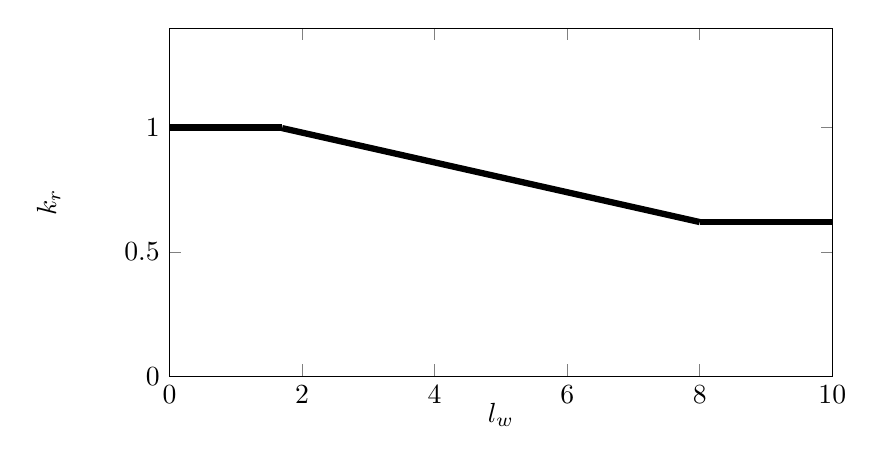
\begin{tikzpicture}
\begin{axis}[
width=10cm,height=6cm,
xlabel=$l_w$,
ylabel=$k_r$,
x label style={at={(axis description cs:0.5,-0.05)},anchor=north},
y label style={at={(axis description cs:-0.15,.5)},anchor=south},
xmin=0,
ymin=0,
xmax=10,
ymax=1.4,
]
\addplot[domain=0:1.7,samples=2,line width=.8mm]({x},1);
\addplot[domain=1.7:8,samples=2,line width=.8mm]({x},{1.1-.06*x});
\addplot[domain=8:10,samples=2,line width=.8mm]({x},.62);
\end{axis}
\end{tikzpicture}